\documentclass{article}


%% Packages
\usepackage{algorithm}% http://ctan.org/pkg/algorithm
\usepackage{algpseudocode}% http://ctan.org/pkg/algorithmicx
\usepackage{amsmath} % gathered
\usepackage{amssymb} % mathbb
\usepackage{authblk}
\usepackage[doi=false,isbn=false,url=false,eprint=false, backend=bibtex, maxbibnames=99,firstinits=true]{biblatex}
\usepackage{blindtext}
\usepackage{bm} % mathbb
\usepackage{color}
\usepackage{float}
\usepackage[margin=0.8in,]{geometry} % Make margins 0.8in inch
\linespread{1.25} % Use 1.5 linespacing (\linespread{x} standard is 1.2, 1.2*x = 1.5 => x = 1.25)
\usepackage{graphicx} % Include images
\usepackage{graphics}
\usepackage{hyperref} % Use hpyerlinks
\usepackage{nomencl}
\makenomenclature
\usepackage{etoolbox}
\renewcommand\nomgroup[1]{%
	\item[\bfseries
	\ifstrequal{#1}{P}{Physics constants}{%
		\ifstrequal{#1}{N}{Number sets}{%
			\ifstrequal{#1}{O}{Other symbols}{}}}%
	]}
\usepackage{subcaption} 





%% Defs
\renewcommand\Affilfont{\fontsize{9}{10.8}\itshape}
\renewcommand{\d}{\text{d}}

\newcommand{\tr}{\text{tr}}
\newcommand{\der}[2]{\dfrac{\text{d} #1}{\text{d} #2}}
\newcommand{\pder}[2]{\dfrac{\partial #1}{\partial #2}}
\newcommand{\sig}{\bm{\sigma}}
\newcommand{\bsig}{\bar{\bm{\sigma}}}
\newcommand{\hsig}{\hat{\bm{\sigma}}}
\newcommand{\eps}{\varepsilon}
\newcommand{\beps}{\bar{\bm{\varepsilon}}}
\newcommand{\heps}{\hat{\bm{\varepsilon}}}
\newcommand{\Eeff}{E_{\text{eff}}}
\newcommand{\red}[1]{{\color{red}#1}}



\newcommand{\singlefig}[4]{
	\begin{figure}[!htb]
		\centering
		\includegraphics[width=#1\linewidth]{#2}
		\caption{#3}
		\label{fig:#4}
	\end{figure}
}

\newcommand{\doublefig}[4]{
	\begin{figure}[!htb]
		\centering
		\begin{subfigure}{0.48\textwidth}
			\centering 
			\includegraphics[width=\linewidth]{#1} 
			\caption{}
		\end{subfigure}\hfill
		\begin{subfigure}{0.48\textwidth}
			\includegraphics[width=\linewidth]{#2}
			\caption{}
		\end{subfigure}
		
		\caption{#3}
		\label{fig:#4}
	\end{figure}
}

\newcommand{\quadfig}[6]{
	\begin{figure}[!htb]
		\centering
		\begin{subfigure}{0.48\textwidth}
			\centering 
			\includegraphics[width=\linewidth]{#1} 
			\caption{}
		\end{subfigure}\hfil
		\begin{subfigure}{0.48\textwidth}
			\includegraphics[width=\linewidth]{#2}
			\caption{}
		\end{subfigure}
		
		\begin{subfigure}{0.48\textwidth}
			\centering 
			\includegraphics[width=\linewidth]{#3} 
			\caption{}
		\end{subfigure}\hfil
		\begin{subfigure}{0.48\textwidth}
			\includegraphics[width=\linewidth]{#4}
			\caption{}
		\end{subfigure}
		
		\caption{#5}
		\label{fig:#6}
	\end{figure}
}


\newcommand{\quinfig}[8]{
	\begin{figure}[!htb]
		\centering
		\begin{subfigure}{#8\textwidth}
			\centering 
			\includegraphics[width=\linewidth]{#1} 
			\caption{}
		\end{subfigure}\hfil
		\begin{subfigure}{#8\textwidth}
			\includegraphics[width=\linewidth]{#2}
			\caption{}
		\end{subfigure}
		
		\begin{subfigure}{#8\textwidth}
			\centering 
			\includegraphics[width=\linewidth]{#3} 
			\caption{}
		\end{subfigure}\hfil
		\begin{subfigure}{#8\textwidth}
			\includegraphics[width=\linewidth]{#4}
			\caption{}
		\end{subfigure}
		
		\begin{subfigure}{#8\textwidth}
			\includegraphics[width=\linewidth]{#5}
			\caption{}
		\end{subfigure}
		
		\caption{#6}
		\label{fig:#7}
	\end{figure}
}

\newcommand{\hexfig}[8]{
	\begin{figure}[!htb]
		\centering
		\begin{subfigure}{0.31\textwidth}
			\centering 
			\includegraphics[width=\linewidth]{#1} 
			\caption{}
		\end{subfigure}\hfil
		\begin{subfigure}{0.31\textwidth}
			\includegraphics[width=\linewidth]{#2}
			\caption{}
		\end{subfigure}\hfil
		\begin{subfigure}{0.31\textwidth}
			\includegraphics[width=\linewidth]{#3}
			\caption{}
		\end{subfigure}
		
		\begin{subfigure}{0.31\textwidth}
			\centering 
			\includegraphics[width=\linewidth]{#4} 
			\caption{}
		\end{subfigure}\hfil
		\begin{subfigure}{0.31\textwidth}
			\includegraphics[width=\linewidth]{#5}
			\caption{}
		\end{subfigure}\hfil
		\begin{subfigure}{0.31\textwidth}
			\includegraphics[width=\linewidth]{#6}
			\caption{}
		\end{subfigure}
		
		\caption{#7}
		\label{fig:#8}
	\end{figure}
}


\newcommand{\heptfig}[9]{
	\begin{figure}[!htb]
		\centering
		\begin{subfigure}{0.31\textwidth}
			\centering 
			\includegraphics[width=\linewidth]{#1} 
			\caption{}
		\end{subfigure}\hfil
		\begin{subfigure}{0.31\textwidth}
			\includegraphics[width=\linewidth]{#2}
			\caption{}
		\end{subfigure}\hfil
		\begin{subfigure}{0.31\textwidth}
			\includegraphics[width=\linewidth]{#3}
			\caption{}
		\end{subfigure}
		
		\begin{subfigure}{0.31\textwidth}
			\centering 
			\includegraphics[width=\linewidth]{#4} 
			\caption{}
		\end{subfigure}\hfil
		\begin{subfigure}{0.31\textwidth}
			\includegraphics[width=\linewidth]{#5}
			\caption{}
		\end{subfigure}\hfil
		\begin{subfigure}{0.31\textwidth}
			\includegraphics[width=\linewidth]{#6}
			\caption{}
		\end{subfigure}
		
		
		\begin{subfigure}{0.32\textwidth}
			\includegraphics[width=\linewidth]{#7}
			\caption{}
		\end{subfigure}
		\caption{#8}
		\label{fig:#9}
	\end{figure}
}



\graphicspath{{./code/figures/}{./inkscape-figures/}{./lit-figures/}} 
\bibliography{curly-hair.bib}

\title{A 1D constitutive mechanical model that evolves with cyclical loading}
\author[1, 2]{Benjamin Alheit\thanks{alhben001@myuct.ac.za}}
\date{\today}

% \ead{alhben001@myuct.ac.za}\cortext[mycorrespondingauthor]{Corresponding author}


\affil[1]{Centre for Research in Computational \& Applied Mechanics, University of Cape Town, 7701 Rondebosch, South Africa}
\affil[2]{Department of Mechanical Engineering, University of Cape Town, 7701 Rondebosch, South Africa}


%\author[1, 2]{Author A\thanks{Corresponding Author: A.A@university.edu}}
%\author[1]{Author B\thanks{B.B@university.edu}}
%\author[1]{Author C\thanks{C.C@university.edu}}
%\author[2]{Author D\thanks{D.D@university.edu}}

\begin{document}
\maketitle
\begin{abstract}
	Many collagenous tissues with crimp, as well as curly hair, display unusual mechanical behaviour during cyclical loading: the stress--strain relationship stiffness with subsequent loading cycles and, in the case of curly hair, the stress-strain relation evolves from parabolic-like upwards curve to a linear Hookean relation after several loading cycles. What is stranger still is that the unloading curve lies above the loading curve for each cycle, and so, at first glance, it seems that the material breaks the second law of thermodynamics -- it seems like the material causes \textit{negative} dissipation. However, this cannot be the case. Hence, the raised stress--strain curve observed during unloading must be due to the release of initially stored potential energy. With this premise in hand, we construct a material model that stiffens as a result of cyclical loading and complies with the second law of thermodynamics. Additionally, Maxwell-like devices are used to model the evolution of the microstructure and hence mechanical behaviour of the material over time. The model is able to replicate several attributes of the behaviour of curly hair: the stress--strain relation has a linear region followed by a toe region during the first cycle of loading; the behaviour evolves during cyclical loading; and the stress--strain relation `converges' to a linear Hookean relationship after many cycles of loading.
\end{abstract}
\section{Introduction}
This work is motivated by stress-strain test data of cyclical loading of curly hair that is presented in Figure \ref{fig:data}.
\begin{figure}[!htb]
	\centering
	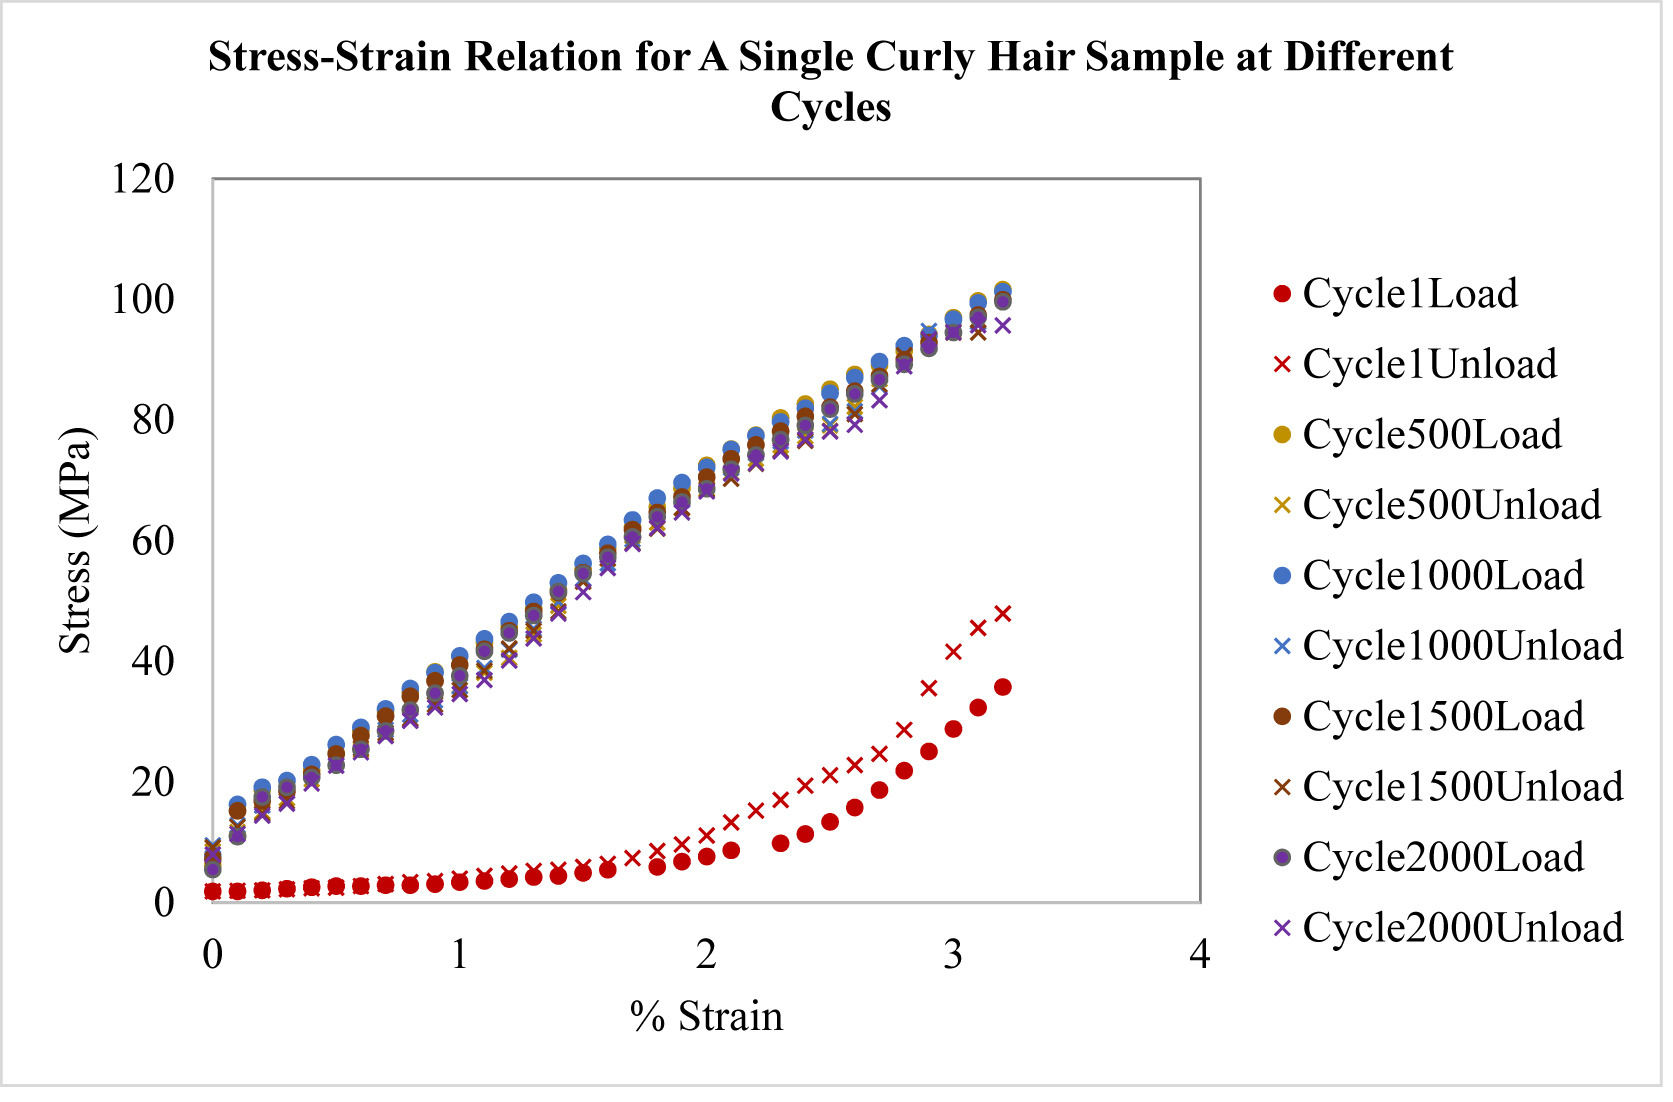
\includegraphics[width=0.6\linewidth]{hair-evolution}
	\caption{Cyclical loading stress-strain data for curly hair \cite{ngoepe2021evolving}.}
	\label{fig:data}
\end{figure}
The stress--strain relationship displays two unusual mechanical characteristics:
\begin{enumerate}
	\item The behaviour stiffens considerably over the loading procedure. Furthermore, it initially has a nonlinear, hyperelastic-like stress-strain relationship, but then progresses to a linear Hookean-like relationship;
	\item The unloading curve for the first cycle (and presumably for many of the cycles prior to the 500$^{\text{th}}$ cycle) is \textit{above} the loading curve. This suggests that the hair does more work on the testing apparatus during unloading than the test apparatus did on the hair during loading.
\end{enumerate}
Hence, at first glance it may seem like the hair is \textit{creating energy} or that it has \textit{negative dissipation}, but this of course is not permitted by the first and second laws of the thermodynamics, respectively. To belabour the point of apparent negative dissipation further, consider the loading curves of an elasto-plastic and viscoelastic material presented in Figures \ref{fig:standard-disp}\,(a) and (b), respectively.
\doublefig{plastic-dissipation}{viscous-dissipation}{Examples of dissipation for (a) an elasto-plastic material \cite{Rub1}, and (b) a viscoelastic material \cite{abramowitch2016introduction}.}{standard-disp}
For both materials the loading curve lies above the unloading curve and the area between them is the dissipation (which must be non-negative due to the second law of thermodynamics). However, for the hair loading behaviour displayed in Figure \ref{fig:data}, the unloading curve is above the loading curve and so the `hysteresis' for the loading cycle is negative. This implies that the change in mechanical behaviour cannot be due to a dissipative procedure, but rather the hair must initially contain stored potential energy that is released during unloading giving rise to the hair doing more work on the testing apparatus during unloading than the apparatus did on the hair during loading.

In what follows, we develop a 1D constitutive model that captures the usual characteristics of the behaviour displayed in Figure \ref{fig:data}. The model is carefully formulated in order to comply with the second law of thermodynamics. 

On a separate matter, we note that similar stiffening behaviour in responses to cyclical loading is observed in soft biological tissues that contain crimp. This has been shown experimentally by means of tests on a synthetic grown collagenous material \cite{susilo2016collagen}, the loading behaviour of which is displayed in Figure \ref{fig:collagen}.
\begin{figure}[!htb]
	\centering
	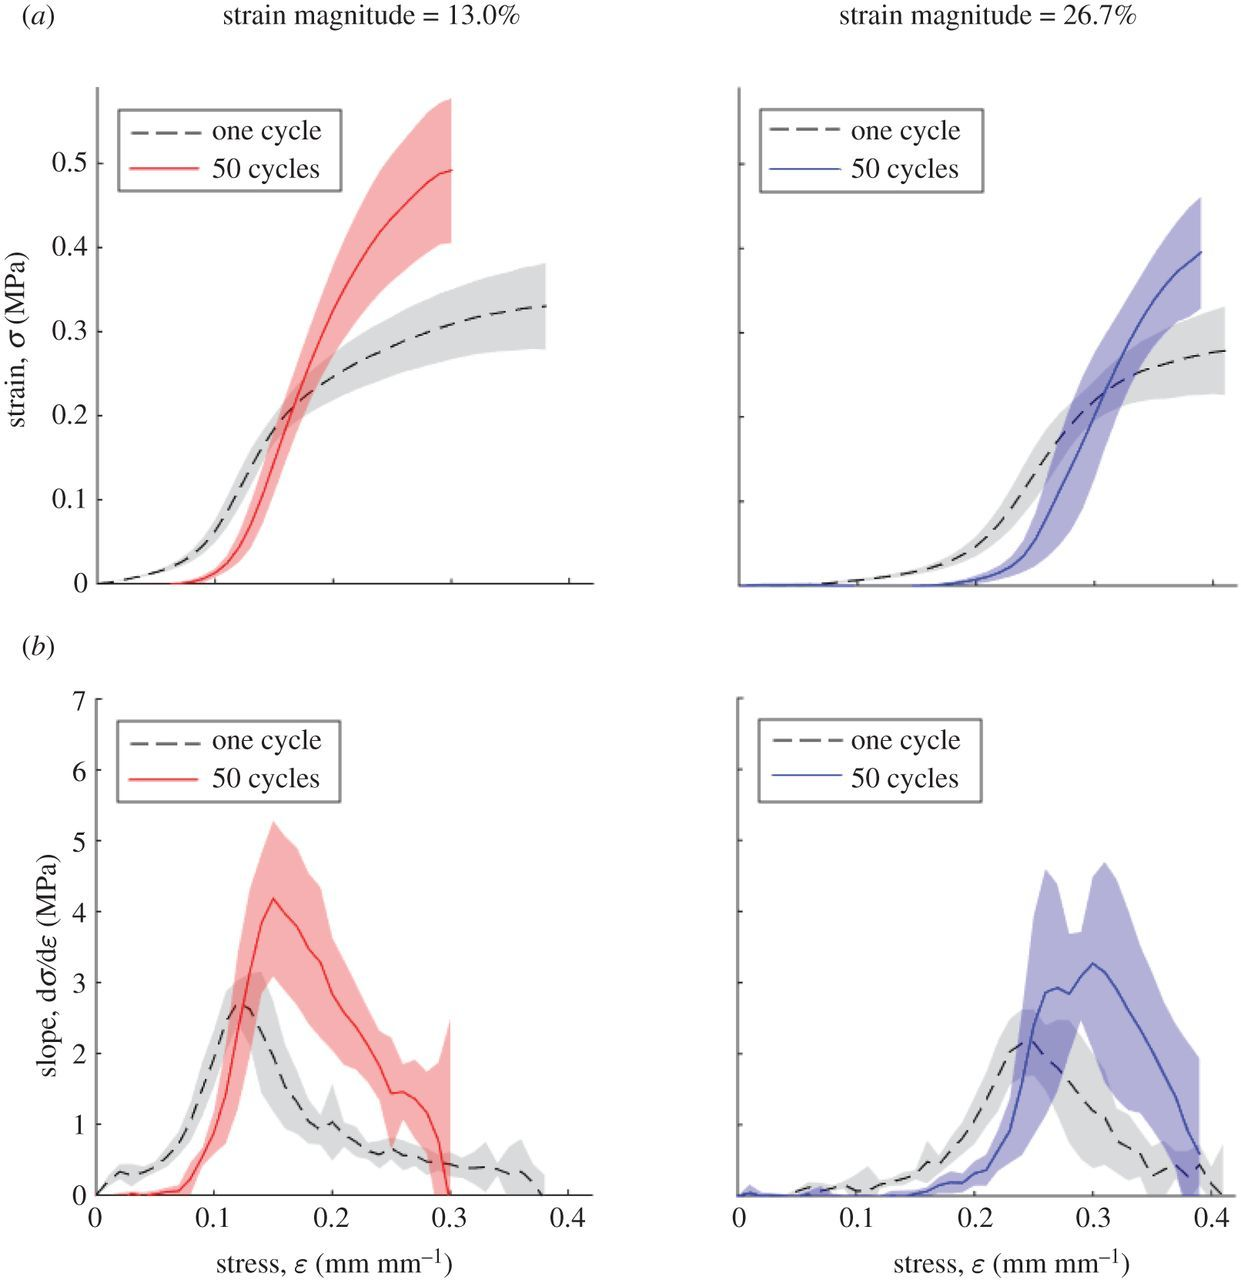
\includegraphics[width=0.7\linewidth]{collagen-stiffening}
	\caption{Stress--strain curves of a collagenous material with crimp for different cycles of loading \cite{susilo2016collagen}. (It seems that the stress and strain axes have been misnamed by the original authors.)}
	\label{fig:collagen}
\end{figure}

\section{A preloaded compound spring model}


\subsection{A compound 1D mechanical device with a single preloaded spring}
To create a material model that stiffens with loading and does not violate the second law of thermodynamics we start by postulating a simple 1D mechanical device, a schematic of which is presented in Figure \ref{fig:single-spring}. 
\quinfig{single-spring-1}{single-spring-2}{single-spring-3}{single-spring-4}{single-spring-5}{Schematic diagrams of a loading cycle of a compound preloaded spring -- a 1D mechanical device. }{single-spring}{0.3}
The device consists of two springs: a base spring with stiffness of $E_b$ and a preloaded spring with a stiffness of $E_{pf}$ that has been preloaded to a strain of $\eps_{pf}$ and is held in place by a fixed latch (Figure \ref{fig:single-spring}\,(a)). We term this a single compound spring device since there is a single preloaded spring. The base spring has a sliding latch connected to the preloaded spring. While the base spring is stretched for values below $\eps_{pf}$ the latch slides frictionlessly along the preloaded spring (Figure \ref{fig:single-spring}\,(b)). Once the base spring reaches a strain of $\eps_{pf}$ the sliding latch fixes itself to the preloaded spring and the fixed latch releases the preloaded spring (Figure \ref{fig:single-spring}\,(c)). As the base spring is stretched further, the initially preloaded spring is stretched with it (Figure \ref{fig:single-spring}\,(d)). Upon releasing the springs they go back to their undeformed state (they are of equal length) and the initially preloaded spring does not reattach to the fixed latch and remains attached to the base spring (Figure \ref{fig:single-spring}\,(e)).

The constitutive model that this device represents is as follows. The stress $\sigma$ is related to the strain $\eps$ by
\begin{equation}
	\sigma = \Eeff \eps\,,
	\label{eq:stress-start}
\end{equation}
where $\Eeff$ is composed of the base stiffness $E_b$ and the preloaded stiffness $E_p$; that is,
\begin{equation}
	\Eeff\left(\gamma\right) = E_b + E_p\left(\gamma\right)\,.
	\label{eq:Eeff}
\end{equation}
The preloaded stiffness depends on the loading history of the device and is given by
\begin{equation}
	E_p\left(\gamma\right) = \begin{cases}
		0 & \gamma < \varepsilon_{pf}\,, \\
		E_{pf} & \gamma \geq \varepsilon_{pf}\,,
	\end{cases}
\end{equation}
where $\gamma$ is the maximum strain that the device has experienced in its loading history; that is, a state variable. Mathematically, this is given by
\begin{equation}
	\gamma = \max_{T\in[0, \,t]} \int^{T}_{0} \dot{\varepsilon} \,\d s \,,
		\label{eq:stress-end}
\end{equation}
where $t$ is the current time and $\dot{\bullet}$ denotes the material time derivative. The resulting stress--strain curves for a single and double loading cycle of such a device are presented in Figures \ref{fig:single-spring-load}\,(a) and (b), respectively.
\doublefig{single-spring-1-cycle}{single-spring-2-cycles}{Loading cycle for a single compound spring mechanical device.}{single-spring-load}
The material parameters used for the model in this case are presented in Table \ref{tab:singl-params}.
\begin{table}
	\centering
	\caption{Material parameters for single compound spring device.}
	\label{tab:singl-params}
	\begin{tabular}{c| c| c}
		$E_b$ (Pa)& $E_{pf}$  (Pa)& $\eps_{pf}$ \\
		\hline \hline
		0.1 & 1 & 1
	\end{tabular}
\end{table}
Note that the second loading cycle is collinear with the unloading curve of Cycle 1 in Figure \ref{fig:single-spring-load}\,(b). This behaviour would continue for all subsequent loading cycles.

\subsubsection{Thermodynamic considerations}
It is clear from Figure \ref{fig:single-spring-load} that the material model stiffens based on its loading history (the unloading curve is above the loading curve), which is what we want to achieve. However, we are yet to show that this model complies with the second law of thermodynamics. It is perhaps obvious that there should be no dissipation (neither positive, nor negative) since the device consists purely of elastic (non-dissipative) springs. However, we prove this here for the sake of rigour. For an isothermal solid in a small--strain 1D setting the Clausius--Duhem inequality (a stronger form of the second law of thermodynamics) is given by
\begin{equation}
	\dot{D} = \sigma \dot{\eps} - \dot{\Psi} \geq 0\,,
\end{equation}
where $\dot{D}$ is the rate of dissipation per unit volume (which must be non-negative) and $\Psi$ is the stored strain energy per unit volume. The strain energy of the device illustrated in Figure \ref{fig:single-spring} is given by
\begin{equation}
	\Psi = \begin{cases}
		\tfrac{1}{2}\left[E_{b}\eps^{2} + E_{pf}\eps_{pf}^{2}\right] & \gamma < \varepsilon_{pf}\,,\\
		\tfrac{1}{2}\left[E_{b} + E_{pf}\right]\eps^{2} & \gamma \geq \varepsilon_{pf}\,,
	\end{cases}
\end{equation}
which is obvious from elementary mechanics. Note that in the initial undeformed state of the device it contains strain energy due to the preloaded spring; that is, $\Psi|_{t=0}=\tfrac{1}{2}E_{pf}\eps_{pf}^{2}$. The time derivative of the strain energy is given by
\begin{equation}
	\dot{\Psi} = \begin{cases}
		E_{b}\eps \dot{\eps}   & \gamma < \varepsilon_{pf}\,,\\
		\left[E_{b} + E_{pf}\right]\eps \dot{\eps} & \gamma \geq \varepsilon_{pf}\,,
	\end{cases}
\end{equation}
and, from equations \eqref{eq:stress-start}--\eqref{eq:stress-end}, the stress of the device is given by 
\begin{equation}
	\sigma = \begin{cases}
		E_{b}\eps    & \gamma < \varepsilon_{pf}\,,\\
		\left[E_{b} + E_{pf}\right]\eps  & \gamma \geq \varepsilon_{pf}\,.
	\end{cases}
\end{equation}
Hence, it is clear that the rate of dissipation of the device is identically zero by the following mathematical development:
\begin{equation}
	\dot{D} = \sigma \dot{\eps} - \dot{\Psi} = \begin{cases}
		E_{b}\eps \dot{\eps} - E_{b}\eps \dot{\eps}  & \gamma < \varepsilon_{pf}\\
		\left[E_{b} + E_{pf}\right]\eps \dot{\eps} - \left[E_{b} + E_{pf}\right]\eps \dot{\eps}  & \gamma \geq \varepsilon_{pf}
	\end{cases} = \begin{cases}
	0  & \gamma < \varepsilon_{pf}\\
	0  & \gamma \geq \varepsilon_{pf}
\end{cases} =0 \geq 0\,.
\end{equation}

Hence, we have achieved the initial goal: the creation of a material model that stiffens based on its loading history and complies with the second law of thermodynamics. This is done by introducing initial stored potential strain energy in the device which is released during unloading which is required for reasons discussed in the introduction.

However, the stress--strain relationship of this model is still far from that displayed in Figure \ref{fig:data}. The discrepancies are as follows:
\begin{enumerate}
	\item The stiffening in Figure \ref{fig:data} occurs in a smooth gradual manner whereas the stiffening in Figure \ref{fig:single-spring} consists of a large single jump;
	\item The stiffening in Figure \ref{fig:data} is gradual not only in response to strain but also in response to time as it occurs over multiple loading cycles whereas the stiffening in Figure \ref{fig:single-spring-load} depends only on the strain history and not on time;
	\item The maximum stress during the first loading cycle of the model is equal to the maximum stress for all loading cycles, whereas the maximum stress in Figure \ref{fig:data} increases with each loading cycle.
\end{enumerate}
In what follows, we attempt to remedy these discrepancies .
\subsection{A compound 1D mechanical device with $n$ preloaded springs}
We can alter the loading path by adding additional springs that are preloaded to different initial strains. As an example, we show a schematic of a loading cycle for a double compound spring device in Figure \ref{fig:double-spring}. 
\heptfig{double-spring-1}
{double-spring-2}
{double-spring-3}
{double-spring-4}
{double-spring-5}
{double-spring-6}
{double-spring-7}
{Loading cycle of a double compound preloaded spring device.}
{double-spring}
Once the base spring is loaded past the initial strain of the bottom preloaded spring, $\tfrac{1}{2}\eps_{pf}$, it latches to the bottom preloaded spring (Figures \ref{fig:double-spring} (a)--(d)). The case is similar for the top preloaded spring (Figures \ref{fig:double-spring} (d)--(f)). Upon unloading, both springs that were initially preloaded remain attached to the base spring (Figure \ref{fig:double-spring} (g)). 

The constitutive behaviour of the device is still described by equations \eqref{eq:stress-start}, \eqref{eq:Eeff}, and \eqref{eq:stress-end}. However, the equation for $E_p$ is different in this case. For the case of two springs, as displayed in Figure \ref{fig:double-spring}, $E_p$ is given by
\begin{equation}
	E_p\left(\gamma\right) = \begin{cases}
		0 & \gamma < \tfrac{1}{2} \varepsilon_{pf} \\
		\tfrac{1}{2}E_{pf} & \gamma \geq \tfrac{1}{2} \varepsilon_{pf}
	\end{cases} + \begin{cases}
	0 & \gamma <  \varepsilon_{pf} \\
	\tfrac{1}{2}E_{pf} & \gamma \geq  \varepsilon_{pf}
\end{cases}\,.
\end{equation}
This can be generalized to the case of $n$ springs by the following equation:
\begin{equation}
	E_p\left(\gamma\right) = \sum_{i=1}^{n}\begin{cases}
		0 & \gamma < \varepsilon_{pf}\dfrac{i}{n} \\
		\dfrac{E_{pf}}{n} & \gamma \geq \varepsilon_{pf}\dfrac{i}{n}
	\end{cases}\,.
\label{eq:n-springs}
\end{equation}
We can now motivate the choice of notation $E_{pf}$ and $\eps_{pf}$: according to equation \eqref{eq:n-springs}, $\eps_{pf}$ is the final strain at which all the preloaded springs have attached to the base spring and $E_{pf}$ is the accumulative stiffness contribution from the preloaded springs $\left(n\dfrac{E_{pf}}{n}=E_{pf}\right)$.

Loading curves where the stiffness due to the preloaded springs is governed by equation \eqref{eq:n-springs} are displayed in Figures \ref{fig:multi-springs}\,(a)--(d) for $n=1,2,10,1000$, respectively. The material parameters are as presented in Table \ref{tab:singl-params}.

\quadfig{spring-1}{spring-2}{spring-10}{spring-1000}{Loading cycle for a compound spring mechanical device with multiple preloaded springs: (a) $n=1$, (b) $n=2$, (c) $n=10$, and (d) $n=1000$.}{multi-springs}

\subsubsection{Infinite preloaded springs}
Until this point, the model stiffens in a discrete manner: it stiffens due to a finite number of springs $n$ that each have a finite stiffness $\dfrac{E_{pf}}{n}$ and engage at a finite number of strains. One may obtain a smooth version of this model is by letting $n\rightarrow \infty$ in equation \eqref{eq:n-springs}. Then, one can obtain the following relation between an increment in $E_{p}$ and $\gamma$\footnote{I have derived this on paper but I omit the details here.}:
\begin{equation}
	\d E_{p} = \begin{cases}
		\dfrac{E_{pf}}{\eps_{pf}}\d \gamma & 0 \leq \gamma \leq \eps_{pf}\\
		0 & \eps_{pf} < \gamma
	\end{cases}\,.
\label{eq:smooth-increments}
\end{equation}
Dealing only with the first case gives
\begin{equation}
	E_{p} = \int_{0}^{t}\dfrac{E_{pf}}{\eps_{pf}}\dot{\gamma}\,\d s = \dfrac{E_{pf}}{\eps_{pf}} \gamma\,.
\end{equation}
Once $\gamma$ has accumulated such that $\gamma=\eps_{pf}$ we have 
\begin{equation}
	E_{p} = E_{pf}\,.
\end{equation}
Then, for any further increase in $\gamma$ we have $\d E_p=0$. Hence, $E_p$ is given by
\begin{equation}
	E_{p} = \begin{cases}
	\dfrac{E_{pf}}{\eps_{pf}} \gamma & 0 \leq \gamma \leq \eps_{pf}\\
	E_{pf} & \eps_{pf} < \gamma
\end{cases}\,.
\end{equation}

Transitioning from these discrete models to a smooth counterpart is important if one creates an analogous 3D model to be implemented in a numerical solver (finite elements, for instance). This would be useful for modelling the evolving mechanical behaviour of soft tissues with crimp. The smooth version of the model is necessary to allow the use of standard calculus tools to derive stress tangents required for numerical solution procedures, such as Newton's method. We show the transition here only to illustrate that it is possible. For the remainder of this document, we continue to use the discrete version of the model and make $n$ large to give an approximation of the equivalent smooth model behaviour where desired, note that this is the case for Figure \ref{fig:multi-springs}\,(d) where $n=1000$ and the loading curve appears smooth to the human eye. 

On another matter, at this point we can provide a somewhat mechanistic motivation for the mathematical form of the model (albeit retroactively). The changing mechanical behaviour of the hair (or soft tissue) must be due to evolution of the microstructure. We assume that, during the evolution, intermolecular bounds form and structural proteins (whether it be collagen or keratin filaments)  become better aligned to bare load. Hence, the model approximates the creation of a new intermolecular bonds or a slight improvements in alignment of a structural protein as the release of a preloaded spring with an infinitesimal stiffness. 

With this motivation in hand, we address two discrepancies the current model has with the data presented in Figure \ref{fig:data}:
\begin{enumerate}
	\item The loading portion of the current model (Figure \ref{fig:multi-springs}) curves upwards from the start --  it does not show an initial linear region followed by a toe region;
	\item The evolution of the mechanical behaviour occurs instantaneously instead of over multiple loading cycles.
\end{enumerate}

\subsubsection{Changing the shape of the loading curve: redistribution of the preloaded springs}
The first discrepancy can be addressed by postulating that more intermolecular bonds are formed closer to the end of the loading cycle. This amounts to a redistribution of the springs so that they are not linearly spaced, rather there is an increasing number of springs further to the right of the loading curve. This is modelled by introducing material parameter $a$ to change the expression for $E_p$ as follows:
\begin{equation}
	E_p\left(\eps\right) = \sum_{i=1}^{n}\begin{cases}
		0 & \gamma < \varepsilon_{pf}\dfrac{i^{a}}{n^{a}} \\
		\dfrac{E_{pf}}{n} & \gamma \geq \varepsilon_{pf}\dfrac{i^{a}}{n^{a}}
	\end{cases}
\label{eq:springs-redistribute}
\end{equation}
Note that equation \eqref{eq:springs-redistribute} is a more general expression for \eqref{eq:n-springs} since equation \eqref{eq:springs-redistribute} reduces to \eqref{eq:n-springs} for $a=1$. We display the loading behaviour for $a=0.2$ with $n=2,5,10,1000$ in Figures \ref{fig:a-multi-springs-n}\,(a)--(d), respectively.
\quadfig{a-02-n-2}{a-02-n-5}{a-02-n-10}{a-02-n-1000}{Loading cycle for a compound spring mechanical device with multiple preloaded springs distributed to the right as per equation \eqref{eq:springs-redistribute} ($a=0.5$): (a) $n=1$, (b) $n=2$, (c) $n=10$, and (d) $n=1000$.}{a-multi-springs-n}
It is clear that making $a$ less than 1 shifts the distribution of the preloaded springs to the right.

Note that the smooth version of equation \eqref{eq:springs-redistribute} ($n\rightarrow\infty$) is not the same as in equation \eqref{eq:smooth-increments} -- it would need to be re-derived.

We also display the loading behaviour for $n=1000$ and $a=1,0.5,0.1,0.05$ in Figures \ref{fig:a-multi-springs}\,(a)--(d), respectively.
\quadfig{a-1-n-1000}{a-05-n-1000}{a-01-n-1000}{a-005-n-1000}{Loading cycle with $n=1000$ for various values of $a$: (a) $a=1$, (b) $a=0.5$, (c) $a=0.1$, and (d) $a=0.05$.}{a-multi-springs}
The linear-to-toe region loading behaviour of the model has been resolved. The next discrepancy to resolve is the evolution of the mechanical behaviour due to cyclical loading.

\subsection{A compound preloaded spring device with evolving latches}

So far we have modelled microstructural changes (the creation of intermolecular bounds and realignment of structural proteins) as the addition of preloaded springs with small stiffness. However, these changes have been modelled to occur instantaneously. Physically we know that this is not the case -- biological tissues evolve over time with loading. Additionally, this microstructural evolution involves sliding of cells and molecules over one another which gives rise to viscous dissipation. Hence, the model ought to be extended to capture evolution occurring over time and include the resulting viscous dissipation. Naturally, this implies that dashpots should be added to the mechanical device. 

This is done by adding a Maxwell-like element to the latch which was previously fixed as illustrated in Figure \ref{fig:evolving2-springs}. 
\hexfig{evolving-1}{evolving-2}{evolving-3}{evolving-4}{evolving-5}{evolving-6}{Loading cycle of a compound spring with an evolving latch.}{evolving2-springs}
The spring of the Maxwell device is preloaded to a strain of $\eps_{pf}$ and, while the preloaded spring with stiffness $E_{pf}$ is attached to the latch of the Maxwell device, the latch is fixed (Figure \ref{fig:evolving2-springs} (a)). Initial loading while $\eps<\eps_{pf}$ behaves as before (Figure \ref{fig:evolving2-springs} (b)). Once the base spring reaches the preloaded spring it latches to it and the Maxwell latch is released -- it is free to evolve (Figure \ref{fig:evolving2-springs} (c)). While $\eps>\eps_{s}$ the Maxwell latch gradually translates left due to the preloading of the Maxwell spring; that is, $\eps_{s}$ gradually decreases and the strain of the dashpot $\eps_{d}$ increases (Figure \ref{fig:evolving2-springs} (d)). Upon unloading, once $\eps$ reaches $\eps=\eps_{s}$, the initially preloaded spring re-latches to the Maxwell latch at a strain of $\eps_{sl}$ and releases the latch from the base spring (Figure \ref{fig:evolving2-springs} (e)). Upon complete unloading, the base spring returns to its undeformed position and the preloaded spring remains latched at a strain of $\eps_{sl}$ (Figure \ref{fig:evolving2-springs} (f)). If the device were to be loaded again the base spring would latch to preloaded spring at a strain of $\eps_{sl}$.

We reiterate here that, although this is a simple phenomenological model it captures numerous attributes that are intuitive about the evolution of the microstructure as well as attributes that are observed in physical tests:
\begin{itemize}
	\item The evolution of the mechanical behaviour (microstructure) is initiated by loading;
	\item The evolution occurs over time -- it is not instantaneous;
	\item The evolution causes dissipation which, intuitively, would occur from the friction between microstructural constituents as they rearrange;
	\item The loading curve contains a toe region which gradually lessens under cyclical loading which is shown in what follows.
\end{itemize}

We now address the mathematics of the model implied by Figure \ref{fig:evolving2-springs}. Although Figure \ref{fig:evolving2-springs} shows only one preloaded spring (apart from the Maxwell spring), we begin immediately with the case for $n$ springs; that is,
\begin{equation}
	E_p\left(\eps\right) = \sum_{i=1}^{n}\begin{cases}
		0 & \eps < \eps_{s}^{(i)} \\
		\dfrac{E_{pf}}{n} & \eps \geq \eps_{s}^{(i)}
	\end{cases}\,.
	\label{eq:springs-evolve}
\end{equation}
Here, $\eps_{s}^{(i)}$ is the current strain of the Maxwell spring for the $i^{\text{th}}$ preloaded spring (the parentheses denotes that $i$ is an index, it is not an exponent). Note that there is no longer a single state variable $\gamma$, rather there is a state variable for each preloaded spring; that is, $\eps_{s}^{(i)}$. To determine how $\eps_{s}^{(i)}$ evolves, we start by using Newton's third law: the forces in the spring and dashpot are equal (or stress if one chooses a unit area for both); that is,
\begin{equation}
	\eta_d \dot{\eps}_{d} = E_{s}\eps_{s}\,.
	\label{eq:n-3}
\end{equation}
For the sake of a cleaner notation we omit the $(i)$. Since both ends of the Maxwell device are fixed, the strain of the spring is equal to the negative of the strain of the dashpot; that is,
\begin{equation}
	\eps_{s} = - \eps_{d}\,, \qquad \dot{\eps}_{s} = - \dot{\eps}_{d}\,.
	\label{eq:strain-equal}
\end{equation}
It is convenient to define the relaxation time as
\begin{equation}
	\tau = \dfrac{\eta_{d}}{E_{s}}\,.
	\label{eq:relax}
\end{equation}
Then, substitution of equations \eqref{eq:strain-equal} and \eqref{eq:relax} into equation \eqref{eq:n-3} gives
\begin{equation}
	\dot{\eps}_{s} + \dfrac{1}{\tau}\eps_{s} = 0\,.
	\label{eq:ode}
\end{equation}
To solve this ODE we introduce the integration factor
\begin{equation}
	\exp\left(\int_{t_r}^{t}\dfrac{1}{\tau}\d t\right) = \exp\left(\dfrac{t-t_{r}}{\tau}\right)\,,
	\label{eq:if}
\end{equation}
where $t_r$ is the time at which the Maxwell latch was released and $t$ is the current time. Multiplication of the integration factor (equation \eqref{eq:if}) on both sides of equation \eqref{eq:ode} gives
\begin{equation}
	\dfrac{\d }{\d t}\left[\eps_{s}\exp\left(\dfrac{t-t_{r}}{\tau}\right)\right] = 0\,.
\end{equation}
We then integrate to obtain
\begin{equation}
	\eps_{s}\exp\left(\dfrac{t-t_{r}}{\tau}\right) = c\,,
\end{equation}
where the constant $c$ is found by using $\eps_{s}\left(t_{r}\right)=\eps_{sl}$. Hence, the evolution of the Maxwell spring is given by
\begin{equation}
	\eps_{s} = \eps_{sl}\exp\left(\dfrac{-(t-t_{r})}{\tau}\right)\,.
	\label{eq:maxwell-evolve}
\end{equation}
An example of this evolution is presented in Figure \ref{fig:es}.
\singlefig{0.5}{es}{Evolution of a single latch driven by a Maxwell element (once the latch has been released) as a function of time.}{es}

Of course, this evolution only occurs while the latch is released. Additionally, initially we have $\eps^{(i)}_{sl} = \varepsilon_{pf}\dfrac{i^{a}}{n^{a}}$. Once a latch is released it evolves according to equation \eqref{eq:maxwell-evolve}, then once $\eps$ crosses the current value for $\eps^{(i)}_{s}$ the last latch strain is set to $\eps^{(i)}_{sl}=\eps^{(i)}_{s}$. Upon reloading, if the strain crosses $\eps^{(i)}_{sl}$ the latch begins to evolve again and $t_r$ is set to the time at which the latch was crossed. 

The behaviour of the model for two cycles of loading is presented in Figures \ref{fig:evolve-multi-springs} (a)--(d) for $n=1,2,10,1000$, respectively. The parameters for the model and loading are given in Table \ref{tab:multi-evolve-params}.
\quadfig{temp-evolution-1}{temp-evolution-2}{temp-evolution-10}{temp-evolution-1000}{Two loading cycles of a compound spring with evolving latches for various preloaded springs: (a) $n=1$, (b) $n=2$, (c) $n=10$, and (d) $n=1000$.}{evolve-multi-springs}
\begin{table}
	\centering
	\caption{Parameters $n$-compound spring device with evolving latches tests.}
	\label{tab:multi-evolve-params}
	\begin{tabular}{c| c| c | c | c | c}
		$E_b$ (Pa)& $E_{pf}$  (Pa)& $\eps_{pf}$ & $a$  & $\tau$ (s) & Cycle time (s) \\
		\hline \hline
		0.1 & 1 & 1 & 0.1 & 3 & 4
	\end{tabular}
\end{table}
Note that, in a sense, the unloading curve is similar to the loading curve but it has been translated to the left. This is due to the latches creeping towards the left. 

The behaviour for 7 loading cycles is when $n=1000$ presented in Figure \ref{fig:cycles-7}.
\singlefig{0.5}{temp-evolution-1000-cycles}{Seven loading cycles of a compound spring with evolving latches with $n=1000$.}{cycles-7}
Note that the model approaches a linear stress--strain relationship after multiple cycles as desired.

\subsubsection{Thermodynamic considerations}
Here we investigate the thermodynamics involved in the evolution of the microstructure and hence of the mechanical behaviour. Although the Maxwell elements alter the mechanical behaviour, they do not contribute to the stress -- their ends are fixed. The springs that contribute to the stress (the base spring and the preloaded springs) do not dissipate energy which has been shown above. Hence, we analyse only the Maxwell elements that drive the evolution of the behaviour. Since the working is the same for each Maxwell element, we omit the $(i)$ superscript so that the notation is cleaner. We require that the model complies with the Clausius-Dunham inequality; that is,
\begin{equation}
	\dot{D} = \sigma_{s} \dot{\eps}_{s} - \dot{\Psi}_{s} \geq 0\,,
	\label{eq:diss}
\end{equation}
where $\sigma_{s}$, $\dot{\eps}_{s}$, and $\dot{\Psi}_{s}$ are the stress, strain rate, and strain energy of the spring in the Maxwell element, respectively. To reiterate, the stress in the Maxwell spring $\sigma_{s}$ does not contribute to the stress defined by the model $\sigma$, it only drives the evolution of the microstructure. The stress in the spring is equal to the stress in the dashpot and is given by
\begin{equation}
	\sigma_{s} = E_{s}\eps_{s} = \eta_{d} \dot{\eps}_{d} \,.
\end{equation}
The strain energy is given by
\begin{equation}
	\Psi = \dfrac{1}{2}E_{s}\eps_{s}^{2}\,.
\end{equation}
However, $\eps_{s}$ implicitly depends on $\eps_{d}$; that is,
\begin{equation}
	\eps_{s} = -\eps_{d}\,.
\end{equation}
Hence, when taking the time derivative of the strain energy one obtains
\begin{equation}
	\begin{aligned}
			\dot{\Psi} &= \pder{\Psi}{\eps_{s}}\dot{\eps}_{s} + \pder{\Psi}{\eps_{d}}\dot{\eps}_{d} \\
			&= \pder{\Psi}{\eps_{s}}\dot{\eps}_{s} + \pder{\Psi}{\eps_{s}}\pder{\eps_{s}}{\eps_{d}}\dot{\eps}_{d}\\
			&= \sigma_{s}\dot{\eps}_{s} - \underbrace{\sigma_{s}}_{\eta_d \dot{\eps}_{d}}\dot{\eps}_{d}\\
			&= \sigma_{s}\dot{\eps}_{s} - \eta_d\dot{\eps}_{d}^{2}\,.
	\end{aligned}
\label{eq:psi-dot}
\end{equation}
Substitution of equation \eqref{eq:psi-dot} into equation \eqref{eq:diss} reveals that the rate of dissipation for a single Maxwell element is given by
\begin{equation}
	\dot{D} =  \eta_d\dot{\eps}_{d}^{2}\geq 0\,.
	\label{eq:diss-positive}
\end{equation}
Hence, we require that $\eta_d\geq 0$ in order to satisfy the second law of thermodynamics (provided that $E_{s}> 0$, this also corresponds to positive relaxation times $\tau$). Recall that, while the latch is released, it evolves according to 
\begin{equation}
	\eps_{s} = \eps_{sl}\exp\left(\dfrac{-(t-t_{r})}{\tau}\right)\,.
\end{equation}
Taking the time derivative of this expression gives
\begin{equation}
	\dot{\eps}_{s} = -\dfrac{\eps_{sl}}{\tau}\exp\left(\dfrac{-(t-t_{r})}{\tau}\right)=-\dot{\eps}_{d}\,.
	\label{eq:es-dot}
\end{equation}
We can then determine the amount of energy dissipated by substitution of equation \eqref{eq:es-dot} into equation \eqref{eq:diss-positive} and integrating over the time for which the latch is free to evolve as follows:
\begin{equation}
	\begin{aligned}
			D &=  \eta_d\dfrac{\eps_{sl}^{2}}{\tau^{2}}\exp\left(\dfrac{2t_{r}}{\tau}\right)\int_{t_r}^{t} \exp\left(\dfrac{-2s}{\tau}\right)\,\d s\\
			&=\eta_d\dfrac{\eps_{sl}^{2}}{\tau^{2}}\exp\left(\dfrac{2t_{r}}{\tau}\right)\left[-\dfrac{\tau}{2}\exp\left(\dfrac{-2t}{\tau}\right)+\dfrac{\tau}{2}\exp\left(\dfrac{-2t_r}{\tau}\right)\right] \\
			& = \dfrac{1}{2}E_{s}\eps_{sl}^{2}\left[1 - \exp\left(-\dfrac{2(t-t_{r})}{\tau}\right)\right]\,.
	\end{aligned}
\end{equation}
An example of the resulting dissipation relation is presented Figure \ref{fig:dissipation}.
\singlefig{0.5}{dissipation}{Dissipation of a single Maxwell element (once the latch has been released) as a function of time.}{dissipation}
The dissipation clearly monotonically increases as time progresses, as required by the second law of thermodynamics. Of course, the total dissipation for the model is sum of the dissipation for each Maxwell element; that is,
\begin{equation}
	D = \sum_{i=1}^{n}\dfrac{1}{2}E_{s}^{(i)}\left[\eps^{(i)}_{sl}\right]^{2}\left[1 - \exp\left(-\dfrac{2(t-t^{(i)}_{r})}{\tau^{(i)}}\right)\right]\,,
\end{equation}
where $\bullet^{(i)}$ denotes a value corresponding to the $i^{\text{th}}$ Maxwell element. Note that each Maxwell element may have different a different value for the parameters $E^{(i)}_{s}$ and $\tau^{(i)}$. However, we choose for them to be the same for the sake of simplicity. 
%Of course, the release time for each element $t_r^{(i)}$ is guaranteed to be different. 

To give an example of the total dissipation experienced over several loading cycles, we repeat the loading conducted to create the stress-strain behaviour presented in Figures \ref{fig:evolve-multi-springs} and \ref{fig:cycles-7}. We use again the parameters presented in Table \ref{tab:multi-evolve-params}. However, we also require values for $E_{s}^{(i)}$. We choose this to be
\begin{equation}
	E_{s}^{(i)}=\dfrac{E_{s}}{n}\,,
\end{equation}
where we choose $E_{s}=1$\, Pa. The corresponding dissipation for the loading shown in Figure \ref{fig:evolve-multi-springs} is displayed in Figure \ref{fig:evolve-multi-springs-dissipation} and the dissipation that corresponds to Figure \ref{fig:cycles-7} is displayed in Figure \ref{fig:disp-cycles-7}.
\quadfig{disp-1}{disp-2}{disp-10}{disp-1000}{Dissipation over time due to microstructural evolution for the corresponding stress--strain curves in Figure \ref{fig:evolve-multi-springs} with (a) $n=1$, (b) $n=2$, (c) $n=10$, and (d) $n=1000$.}{evolve-multi-springs-dissipation}

\singlefig{0.5}{disp-1000-cycles}{Dissipation over time due to microstructural evolution for the corresponding stress--strain curve in Figure \ref{fig:cycles-7}.}{disp-cycles-7}

\section{Conclusion}
The model created (defined by equations \eqref{eq:stress-start}, \eqref{eq:stress-start}, \eqref{eq:springs-evolve}, and \eqref{eq:maxwell-evolve}, with behaviour displayed in Figure \ref{fig:cycles-7}) replicates several attributes displayed by the cyclical loading of curly hair:
\begin{itemize}
	\item The initial loading curve has a toe region;
	\item The unloading curve is above the loading curve;
	\item The behaviour evolves over several loading cycles to eventually replicate a linear Hookean material.
\end{itemize}
Additionally, the model has several attractive attributes from a mechanical perspective:
\begin{itemize}
	\item It complies with the second law of dynamics;
	\item The modelling of the evolution of the microstructure causes dissipation which is physically intuitive. 
\end{itemize}
However, there is still one critical discrepancy between the model and the test data shown in Figure \ref{fig:data}: the maximum stress during the first loading cycle of the model is equal to the maximum stress for all loading cycles, whereas the maximum stress in the data increases with each loading cycle. Clearly the structure of the model needs to be altered to allow for this.

\section{Possible extensions to this work}
The work presented here provides fertile ground for future work. Some possible important and/or interesting extensions to this work include:
\begin{enumerate}
	\item Altering the model so that the maximum stress experienced during a loading cycle increases with the number of loading cycles;
	\item In \cite{ngoepe2021evolving} it is stated that, after cyclical loading, curly hair goes back to its original state upon immersion in water. In the setting of the model presented here this is equivalent to the re-preloading of the preloaded springs. Hence, the water (perhaps due to the presence of free ions) provides stored potential energy to the hair again. It would be interesting to add this remodelling process to the current model;
	\item It would be good to calibrate the model to test data of hair to see if a good fit can be achieved; 
	\item It would also be interesting to see if the model could fit data other than just cyclical loading. For instance, one might apply a loading procedure where a tensile strain is applied and held for some time, the gradually increased and held again, then slowly released, and repeat this process at various strain rates. There are of course infinitely many permutations of loading procedures that could be applied. It would be interesting to see the results of a large number of these and to see if a model could capture the behaviour in all of these scenarios;
	\item I note here that fitting of the material parameters $E_b$, $E_{pf}$, $\eps_{pf}$, $a$, and $\tau$ can be done using stress--strain data. To determine the one remaining material parameter $E_s$ (or, equivalently, $\eta_{d}$ since $\tau$ would be defined by the stress strain curves) one would need dissipation--time data. Dissipation is the transfer of mechanical energy into heat. Hence, to obtain this data, one would need to constantly measure the temperature in the testing set-up to determine the thermal energy that is being released; that is, the dissipation;
	\item If the 5 points above are dealt with, I think this work, in addition to some image data and (as mentioned above) more mechanical test data, would make for a nice publication in Acta Biomaterialia -- they seem to really like the combination of mechanical test data, image data, and a simple mechanical model such as the one presented here;
	\item Once the maximum stress issue is resolved, it would be interesting to construct an analogous 3D model (I have made the transition from 1D viscoelastic models to 3D models before so I am confident that I could do that in this case too);
	\item The 3D model could also include a remodelling process that allows for recrimping of the structural protein fibres (perhaps in response to a supply of biological nutrients);
	\item With a 3D model in hand, it would be useful to obtain cyclical test data of soft collagenous tissue with crimp to calibrate the 3D model to;
	\item I know you (Prof. Ngoepe) do a lot of work in biomechanics -- do you perhaps have connections that could provide us with soft collagenous tissue test samples? Then, perhaps, we could collaborate with the soft tissue experimentalists is BISRU (Reuben) to obtain the relevant test data;
	\item I think the 3D model and related test data (as well as image data) would make for another nice publication, but perhaps in a more mechanics heavy journal than Acta Biomaterialia since the 3D mechanics will be quite involved.
\end{enumerate}

	\printbibliography
\end{document}